%!TeX TS-program = pdflatex
%!TeX encoding = UTF-8 Unicode
%!TeX spellcheck = en-US
%!BIB TS-program = bibtex
% -*- coding: UTF-8; -*-
% vim: set fenc=utf-8
%TODO include changing point theory and bibliography
%%%%%%%%%%%%%%%%%%%%%%%%%%%%%%%%%%%%%%%%%%%%%%%%%%%%%%%%%%%%%%%%%%%%%
\newcommand{\AuthorA}{Chlo\'e Pasturel}
\newcommand{\AuthorB}{Jean-Bernard Damasse}%
\newcommand{\AuthorC}{Anna Montagnini}%
\newcommand{\AuthorD}{Laurent U.~Perrinet}%
\newcommand{\Address}{Institut de Neurosciences de la Timone, CNRS / Aix-Marseille Universit\'e - Marseille, France}%
\newcommand{\Website}{http://invibe.net/LaurentPerrinet}%
\newcommand{\Email}{Laurent.Perrinet@univ-amu.fr}%
\newcommand{\Title}{Estimating and anticipating a dynamic probabilistic bias in visual motion direction}
\newcommand{\Acknowledgments}{ANR grant <<Reinforcement and Eye Movements>> \textbf{ANR-13-APPR-0008-02} - code and material @ \url{\Website/Publications/Pasturel_etal2018} }
\newcommand{\Abstract}{Humans are able to accurately track a moving object with a combination of saccades and smooth eye movements. These movements allow us to align and stabilize the object on the fovea, thus enabling high-resolution visual analysis. When predictive information is available about target motion, anticipatory smooth pursuit eye movements (aSPEM) are efficiently generated before target appearance, which reduce the typical sensorimotor delay between target motion onset and foveation. It is generally assumed that the role of anticipatory eye movements is to limit the behavioral impairment due to eye-to-target position and velocity mismatch.
By manipulating the probability for target motion direction, we were able to bias the direction and mean velocity of aSPEM, as measured during a fixed duration gap before target ramp- motion onset. This suggests that probabilistic information may be used to inform the internal representation of motion prediction for the initiation of anticipatory movements. However, such estimate may become particularly challenging in a dynamic context, where the probabilistic contingencies vary in time in an unpredictable way. In addition, whether and how the information processing underlying the buildup of aSPEM is linked to an explicit estimate of probabilities is unknown. We developed a new paired-task paradigm in order to address these two questions. In a first session, participants observe a target moving horizontally with constant speed from the center either to the right or left across trials. The probability of either motion direction changes randomly in time. Participants are asked to estimate "how much they are confident that the target will move to the right or left in the next trial" and to adjust the cursor's position on the screen accordingly. In a second session the participants eye movements are recorded during the observation of the same sequence of random-direction trials.
In parallel, we are developing new automatic routines for the advanced analysis of oculomotor traces. In order to extract the relevant parameters of the oculomotor responses (latency, gain, initial acceleration, catch-up saccades), we developed new tools based on best-fitting procedure of predefined patterns (i.e. the typical smooth pursuit velocity profile).
}
%%%%%%%%%%%%%%%%%%%%%%%%%%%%%%%%%%%%%%%%%%
\documentclass[profile,final,english, draft]{article}%
\usepackage{babel}
% MATHS (AMS)
\usepackage{amsmath}
\usepackage{amsfonts} 
\usepackage{amssymb}
\usepackage{amsthm}
\newcommand{\KL}[2]{\text{KL}( #1 | #2 )}
%% parenthesis
\newcommand{\pa}[1]{\left( #1 \right)}
\newcommand{\bpa}[1]{\big( #1 \big)}
\newcommand{\choice}[1]{ %
	\left\{ %
		\begin{array}{l} #1 \end{array} %
	\right. }
% ensembles
\newcommand{\ens}[1]{ \{ #1 \} }
\newcommand{\enscond}[2]{ \left\{ #1 \;;\; #2 \right\} }
% egal par définition
\newcommand{\eqdef}{\ensuremath{\stackrel{\mbox{\upshape\tiny def.}}{=}}}
\newcommand{\eqset}{\ensuremath{\stackrel{\mbox{\upshape\tiny set}}{=}}}
\newcommand{\eq}[1]{\begin{equation*}#1\end{equation*}}
\newcommand{\eql}[1]{\begin{equation}#1\end{equation}}

\DeclareMathOperator{\argmin}{argmin}
\DeclareMathOperator{\argmax}{argmax}
\newcommand{\uargmin}[1]{\underset{#1}{\argmin}\;}
\newcommand{\uargmax}[1]{\underset{#1}{\argmax}\;}
\newcommand{\umin}[1]{\underset{#1}{\min}\;}
\newcommand{\umax}[1]{\underset{#1}{\max}\;}
\newcommand{\usup}[1]{\underset{#1}{\sup}\;}
% for units
\usepackage{siunitx}%
\newcommand{\ms}{\si{\milli\second}}%
%% ========  polices de caracteres =============
\usepackage[T1]{fontenc}% 
\usepackage{lmodern}%
\usepackage{t1enc}
\usepackage{ragged2e}
%============ graphics ===================
\usepackage[pdftex]{graphicx}% 
\DeclareGraphicsExtensions{.pdf,.png,.jpg}%
\graphicspath{{./figures/}}%
%\usepackage[numbers,comma,sort&compress,round]{natbib} %
\usepackage[%style=nature,
maxcitenames=2,
maxnames = 2,
firstinits=true,
uniquename=init,
sorting=none,
url=false,
isbn=false,
eprint=false,
texencoding=latin1,
bibencoding=utf8,
autocite=superscript,
backend=bibtex,
%articletitle=false
]{biblatex}%
\addbibresource{Pasturel_etal2018.bib}%
\newcommand{\citep}[1]{(\cite{#1})}
%\newcommand{\citet}[1]{(\textcite{#1})}
%%%%%%%%%%%%%%%%%%%%%%%%%%%%%%
%% OPTIONAL MACRO FILES
%\usepackage{tikz,tkz-euclide} \usetkzobj{all} % loading all objects
%\usetikzlibrary{positioning} \usetikzlibrary{calc}
%\usepackage{sfmath}
%============ hyperref ===================
\usepackage[unicode,linkcolor=red,citecolor=red,filecolor=black,urlcolor=red,pdfborder={0 0 0}]{hyperref}%
\hypersetup{%
pdftitle={\Title},%
pdfauthor={\AuthorA},%< \Email > \Address},%
}%
\usepackage{color}%
%%%%%%%%%%%%%%%%%%%%%%%%%%%%%%%%%%%
\title{\Title}%
\author{\AuthorA, 
%\AuthorB,  
\AuthorC,  \AuthorD\thanks{\Address} }

%%%%%%%%%%%% Her begynner selve dokumentet %%%%%%%%%%%%%%%
\begin{document}%
\maketitle%
%%%%%%%%%%%%%%%%%%%%%%%%%%%%%%%%%%%%%%%%%%%%%%%%%%%%%%%%%%%%%%%%
% Abstract
\begin{abstract}
\Abstract
\end{abstract}

\section{Problematic}

Humans are able to accurately track a moving object with a combination of saccades and smooth eye movements. These movements allow us to align and stabilize the object on the fovea, thus enabling high-resolution visual detection. When predictive information is available about target motion, anticipatory smooth pursuit eye movements (aSPEM) are efficiently generated before target appearance, which reduce the typical sensorimotor delay between target motion onset and foveation. It is generally assumed that the role of anticipatory eye movements is to limit the behavioral impairment due to eye-to-target position and velocity mismatch.

By manipulating the probability for target motion direction we were able to bias the direction and mean velocity of aSPEM, as measured during a fixed duration gap before target ramp-motion onset. This suggests that probabilistic information may be used to inform the internal representation of motion prediction for the initiation of anticipatory movements~\parencite{Montagnini2010}.

%\begin{center}
%\includegraphics[width=1\linewidth]{anna_methode}
%\end{center}



\begin{tabular}{cc} 
    \includegraphics[width=.49\linewidth]{image_anna_1} & 	\includegraphics[width=.49\linewidth]{image_anna_2}
\end{tabular}
%\vspace{0.5cm}
%\begin{center}
%\includegraphics[width=0.9\linewidth]{image_anna_1}
%\end{center}
%\vspace{0.5cm}
%\begin{center}
%\includegraphics[width=0.9\linewidth]{image_anna_2}
%\end{center}

However, such estimate may become particularly challenging in a dynamic context, where the probabilistic contingencies vary in time in an unpredictable way. In addition, whether and how the information processing underlying the buildup of aSPEM is linked to an explicit estimate of probabilities is unknown.


\section{Material and Method}

In order to answer these questions, we have set up an experiment comprising 3 blocks of 200 trials. For each trial, a target makes either to the left or to the right, this direction being drawn from a Bernoulli process. The probability of this process varied in a piecewise-constant (that is, a step function varying between~$0$ and~$1$), similarly to~\textcite{Meyniel13}. The occurence of these switches is itself drawn from a Bernoulli process of probability $p_{switch}=1/40$.

%-------------------------------------------------------------%
%: fig: protocole
\begin{figure}[b!]
%\vspace{2mm}
\begin{center}
     \includegraphics[width=.49\linewidth]{materiel_bet}
    \includegraphics[width=.49\linewidth]{materiel_recording}

    \includegraphics[width=1\linewidth]{exp}
\end{center}
\caption{\emph{Protocol and previous results} \textbf{(A)} 
\textbf{(B)} 
\textbf{(C)}  }
\label{fig:warps}
\end{figure}
%-------------------------------------------------------------%

We asked subjects to perform two tasks on different days :
%\begin{itemize}\setlength{\itemsep}{0ex}
%\item a <<Bet>>
%\item a <<recording>>
%\end{itemize}

\subsection{The Bet}
In this first part, the subjects must simply answer before each trial at the question \textit{ ``How sure are you that the target will go left or right''}. This was performed by adjusting a cursor on the screen using the mouse (see Figure).

%\subsection{The Bet}
%Example of results obtained during the bet :
%\begin{center} 
%    \includegraphics[width=1\linewidth]{results_pari}
%\end{center}
%%Comparison of probabilities bet with respect to the real probability :
%The scatter plot of the value of the bet (probability bet) as a function of the real probability at every given trial shows that there is a good correlation between both values:

%\begin{center}
%    \includegraphics[width=1\linewidth]{p_real--p_bet}
%\end{center}

\subsection{Eye movements recording}
Then, we recorded their eye movements as they were tracking the target's motion. Importantly, we used that exact same sequence.

%
Stimuli were generated using Matlab 7.10.0 on a Mac running OS 10.6.8 and displayed on a 20" Viewsonic p227f monitor with resolution $1024\times 768$ at 100~\si{\Hz}. Psychophysics routines were written using Matlab and Psychtoolbox 3.0.9 controlled the stimulus display. Observers sat 57~\si{\cm} from the screen in a dark room. Six male observers with normal or corrected-to-normal vision took part in these experiments. They gave their informed consent and the experiments received ethical approval from the Aix-Marseille Ethics Committee in accordance with the declaration of Helsinki.


\subsection{Eye movements analysis}

In order to extract the relevant parameters of the oculomotor responses, we developed new tools based on a best-fitting procedure of predefined patterns and in particular the typical smooth pursuit velocity profile that was recorded for the aSPEM (Top row). This was applied to each trial individually, and we show below some prototypical example of respectively a neutral, anticipatory positive and anticipatory negative aSPEMs examples (respectively second to bottom rows) :

\begin{center} 
    \includegraphics[width=1\linewidth]{Fonction_Fit}
    \includegraphics[width=1\linewidth]{Fit_vitesse}
\end{center}

\section{Results}


\section{Results}

\subsection{Eye movements recording and the Bet}
%Example of results obtained during the recording overlaid with the results of the bet experiment :

Example of results obtained during the bet and the recording :

\begin{center}
    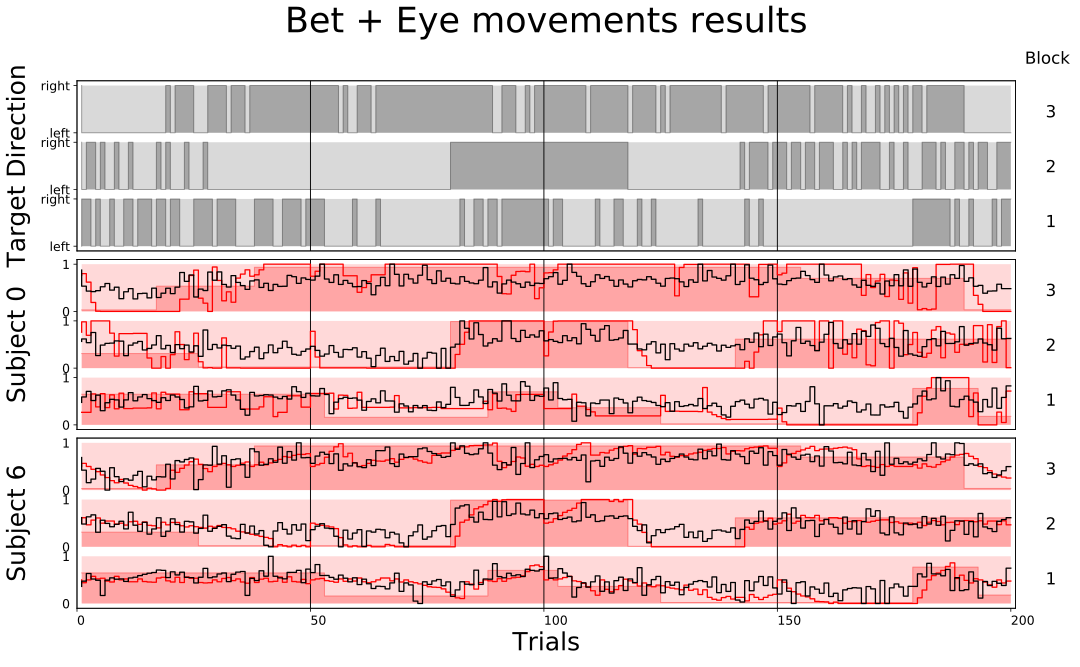
\includegraphics[width=1\linewidth]{results_enregistrement}
\end{center}

%Let's plot the acceleration of anticipation (slope of aSPEM) as a function of the real probability at every given trial :

%\begin{center} 
%    \includegraphics[width=1\linewidth]{p_real--v_a}
%\end{center}

Let's plot the value of the bet (probability bet)  and the acceleration of anticipation (slope of aSPEM) as a function of the real probability at every given trial :

\begin{center} 
    \includegraphics[width=1\linewidth]{P_real}
\end{center}

Which give a strong and positive Pearson coefficient.

\subsection{Relating the Bet to the Recording}

We now compare the value of bet during the bet experiment with the acceleration of anticipation during the recording :

%\begin{center} 
%    \includegraphics[width=1\linewidth]{p_parie--v_a}
%\end{center}

\begin{center} 
    \includegraphics[width=1\linewidth]{p_bet--v_a}
\end{center}


\section{Model}

\subsection{Bayesian change point model}

We have designed an agent adapted the Bayesian Online Change-point Detection model~\parencite{AdamsMackay2007}. This model uses a latent variable r which represents the length of the current interval during which motion-direction probability ($\hat{P}$) has not changed. The agent infers at each trial the likelihood  of r and then deduces the optimal $\hat{P}$ (we used the expected value and the max as readouts) and the uncertainty associated to it. We simulated the model across our experimental sequences, as illustrated by the example for the third block.


\begin{center} 
    \includegraphics[width=1\linewidth]{bayesianchangepoint}
\end{center}

%\begin{center} 
%    \includegraphics[width=1\linewidth]{bayesianchangepoint_e}
%\end{center}

%\begin{center} 
%    \includegraphics[width=1\linewidth]{bayesianchangepoint_m}
%\end{center}


\subsection{Bayesian change point}

where $\KL{\hat p}{p}$ is the Kullback-Leibler divergence between samples $\hat p$ and model $p$ under a Bernouilli distribution
\begin{equation}
\KL{\hat p}{p} = \hat{p} \log\pa{\frac{\hat p}{p}} + (1-\hat p) \log\pa{\frac{1-\hat p}{1-p}}.
\end{equation}

  
\subsection{Comparing the Bayesian change point model with humans}

We now compare the individual guesses during the bet experiment and the acceleration of anticipation during the eye movement recordings with the model simulations :

\begin{center} 
    \includegraphics[width=1\linewidth]{results_bayesianchangepoint_e}
\end{center}

\begin{center} 
    \includegraphics[width=1\linewidth]{results_bayesianchangepoint_m}
\end{center}



\section{Conclusions}


\begin{itemize}\setlength{\itemsep}{0ex}
\item There is a strong correlation between the real probability and the value of the bet,

\item there is a stong correlation between the strength of anticipation and the probability of the process,

\item we have developed a Bayesian model of an agent estimating the probability of changing points. This allows to dynamically infer the direction probability and directly compare model and human behaviour.

\end{itemize}

{\tiny
\printbibliography
}
%%%%%%%%%%%%%%%%%%%%%%%%%%%%%%%%
\end{document}%
